\documentclass{article}
\usepackage[utf8]{inputenc}
\usepackage[T1]{fontenc}
\usepackage[french]{babel}
\usepackage{amsmath,amsfonts,amssymb,amsthm}
\usepackage[margin=2.5cm]{geometry}
\usepackage{graphicx}

\begin{document}

\paragraph{Introduction}
En ce qui concerne les diagrammes de séquence de l'extension de gestion de cartes. J'ai réaliser
ceux qui était les moins évident. Cependant ils suivent tous plus ou moins le même pattern.

\paragraph{Payer avec une carte}

Cette interaction comment par l'utilisateur qui entre les données nécessaires au paiement
dans la CardPayScene(1). La scène enclenche le payement à l'AbstractCard sélectionnée(2).
\newline
Ensuite:
\begin{itemize}
    \item Soit elle envoie sa demande de paiement(3). Le serveur répond qu'une erreur s'est produite.(4)
    La carte communique qu'une erreur s'est produite à la CardPayScene(5)
    \item Soit elle envoie sa demande de paiement(6). Le serveur répond que le transfer s'est correctement
        effectué. La carte communique que le paiement s'est effectué à la CardPayScene(5)
\end{itemize}
 


\begin{figure}[h!]
    \hbox{
        \centering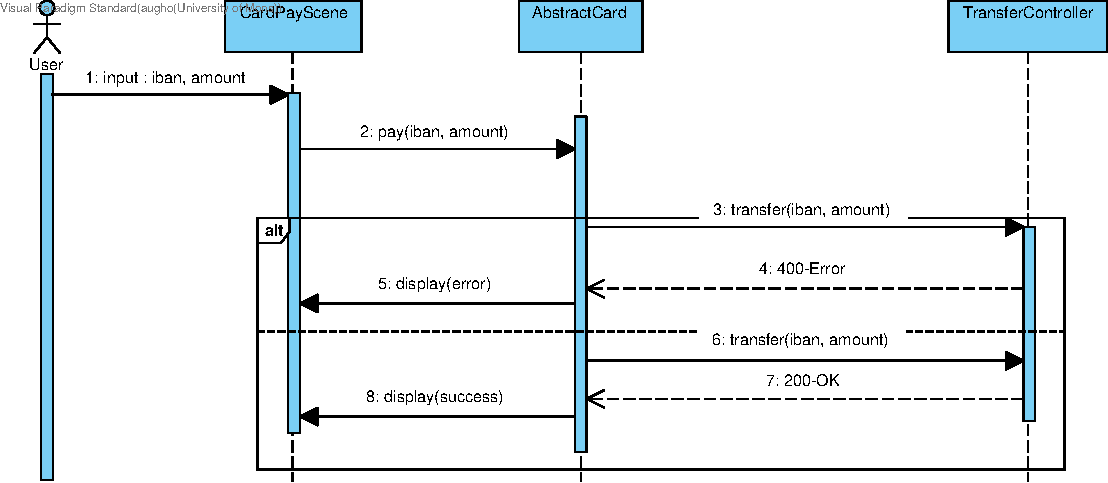
\includegraphics[width=\linewidth]{./img/sequence-client-Extension-1_pay.pdf}
    }
    \caption{Payer avec une carte}
\end{figure}

\newpage

\paragraph{Créer une carte}

\begin{figure}[h!]
    \hbox{
        \centering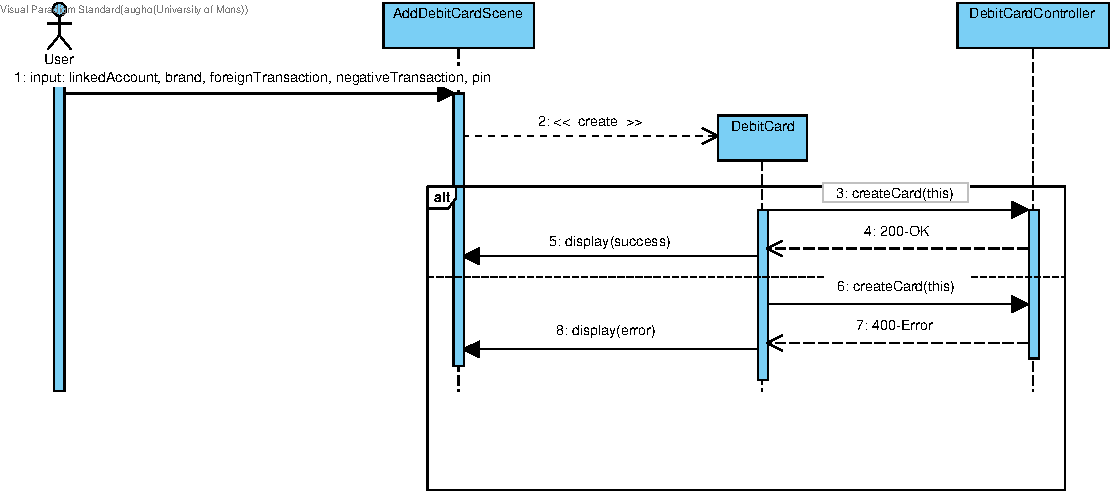
\includegraphics[width=\linewidth]{./img/sequence-client-Extension-1_create.pdf}
    }
    \caption{Créer une carte}
\end{figure}

\newpage

\paragraph{Modifier une carte}

\begin{figure}[h!]
    \hbox{
        \centering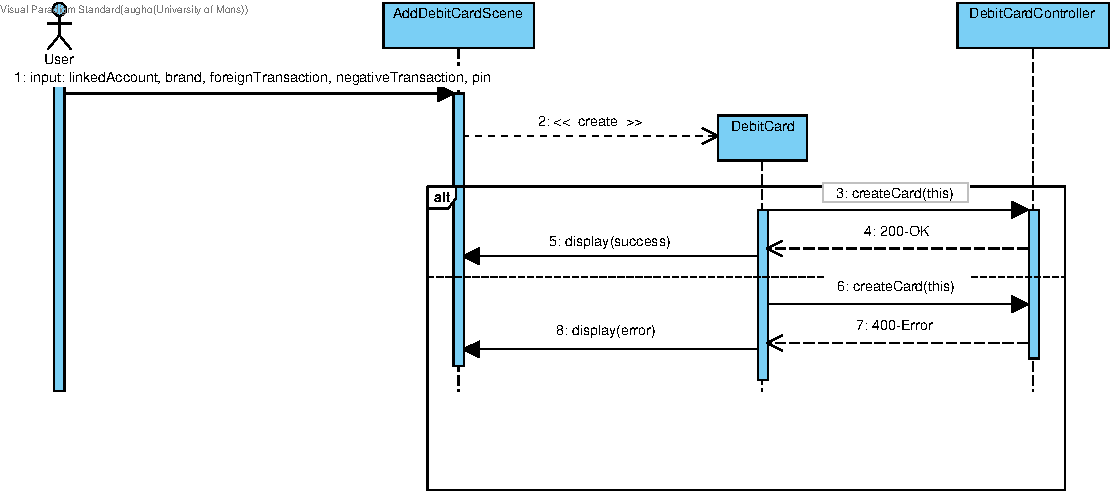
\includegraphics[width=\linewidth]{./img/sequence-client-Extension-1_create.pdf}
    }
    \caption{Modifier une carte}
\end{figure}

\end{document}